\documentclass[a4paper,10pt]{article}

\usepackage{fullpage}
\usepackage[T1]{fontenc}
\usepackage{graphicx}
\usepackage{float}
\usepackage{amsmath}
\usepackage{tabulary}
\usepackage{listings}
\usepackage[spanish]{babel}
\usepackage[utf8]{inputenc}
\usepackage{color}
\usepackage[pdfborder={0 0 0}]{hyperref}
\usepackage{alltt}
\usepackage{moreverb}
\usepackage{enumitem}
\usepackage{array}



% Título principal del documento.`
\begin{document}
\title{	
	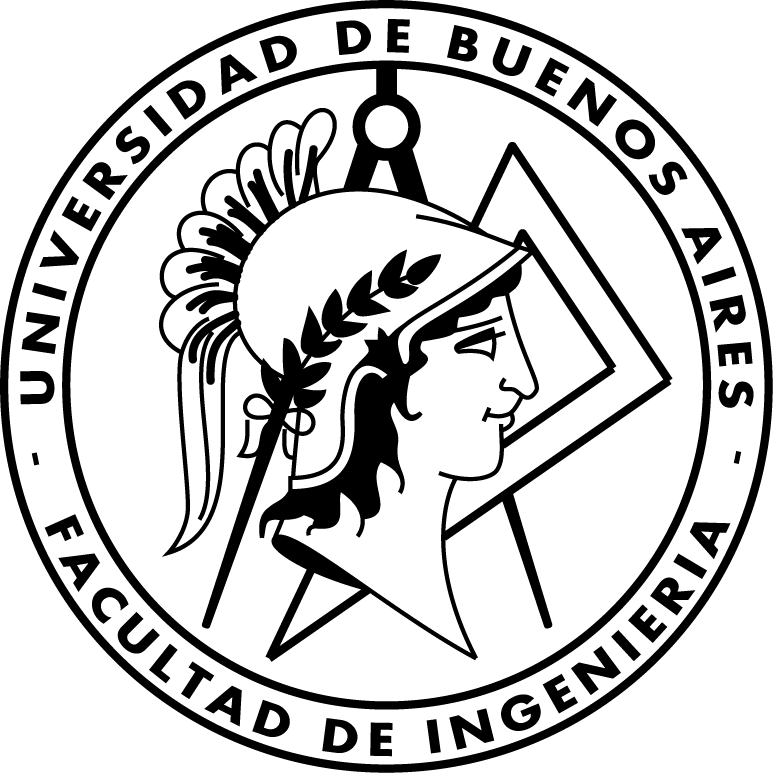
\includegraphics[scale=0.8]{images/logo-fiuba.png} \\
	\begin{center}
		\textbf{Trabajo Práctico N$^{\circ}$3} \linebreak
	\end{center}
	\begin{center}
		\begin{large}
			75.29 - Teoría de Algoritmos I \linebreak
			Facultad de Ingeniería de la Universidad de Buenos Aires \linebreak
			1er. Cuatrimestre 2017 \linebreak
		\end{large}
	\end{center} 
}
\author{	Federico Brasburg, \textit{Padrón Nro. 96.653} \\
			\texttt{ federico.brasburg.@gmail.com } \\ [2.5ex]
			Pablo Rodrigo Ciruzzi, \textit{Padrón Nro. 95.748} \\
			\texttt{ p.ciruzzi@hotmail.com } \\ [2.5ex]
			Andrés Otero, \textit{Padrón Nro. 96.604 } \\
			\texttt{ oteroandres95@gmail.com } \\ [2.5ex] \\
\\
		}
\date{23 de junio de 2017}

\maketitle
\thispagestyle{empty}

\pagebreak 

\tableofcontents
\pagebreak

\clearpage
\section{Programación Dinámica}

\subsection{Cómo correrlo}

\section{Algoritmos Randomizados}

\subsection{Cómo correrlo}

\section{Algoritmos Aproximados}

\subsection{Cómo correrlo}

\pagebreak

\newpage
\section{Código}
\lstset{
	language=Python, columns=flexible, breaklines=true, frame=single, title=creador\_grafos.py
}
\lstinputlisting{../src/creador_grafos.py}

\lstset{ title=grafo.py }
\lstinputlisting{../src/grafo.py}

\lstset{ title=parser.py }
\lstinputlisting{../src/parser.py}

\end{document}